\documentclass[a4paper,12pt]{report}
\usepackage[T2A]{fontenc}
\usepackage{ucs}
\usepackage[utf8x]{inputenc}
\usepackage[english,russian]{babel}
\usepackage{graphicx}
\usepackage{bytefield}
\pagestyle{plain}

\begin{document}
\author{Андриенко Евгений}
\date{02.08.2009}
\title{Описание протокола для взаимодействия между собой системы из терминалов и АРМ.}
\maketitle

Создаваемый сервер должен координировать совместную работу некоторого заранее неизвестного 
количества АРМ\footnote{Автоматизированное Рабочее Место} и терминалов. В создаваемом прикладном 
протоколе необходимо реализовать рассылку пакетов:
\begin{itemize}
\item По адресу -- адрес терминала(АРМ) определяется парой значений IP\_address:port
\item Всем доступным получателям (broadcasting).
\end{itemize}

%---------------------------------------------------------------------------

Список адресов доступных терминалов/АРМ заранее определяется в конфигурационном файле программ для 
АРМ и терминала. Эти же адреса сохраняются при подключении клиента во внутренних структурах данных 
сервера: при помощи них проверяется доступность клиента при попытке отослать ему данные.

%---------------------------------------------------------------------------

Посылаемые пакеты с данными должны быть зашифрованы методом шифрования с открытым ключом\footnote{Можно RSA. Можно использовать библиотеку OpenSSL. http://www.opennet.ru/docs/RUS/use\_openssl/}. У АРМ есть закрытый ключ, которым они расшифровывают сообщения от терминалов, а у терминалов -- 
открытый ключ, которым они зашифровывают данные для АРМ. 
И для пакетов с данными также должна 
быть реализована проверка контрольной суммы.

Максимально возможный размер пакета: 512 Мб.

Все двух- и четырехбайтовые поля в пакете (порт, размер блока данных) должны использовать сетевой 
порядок байтов.

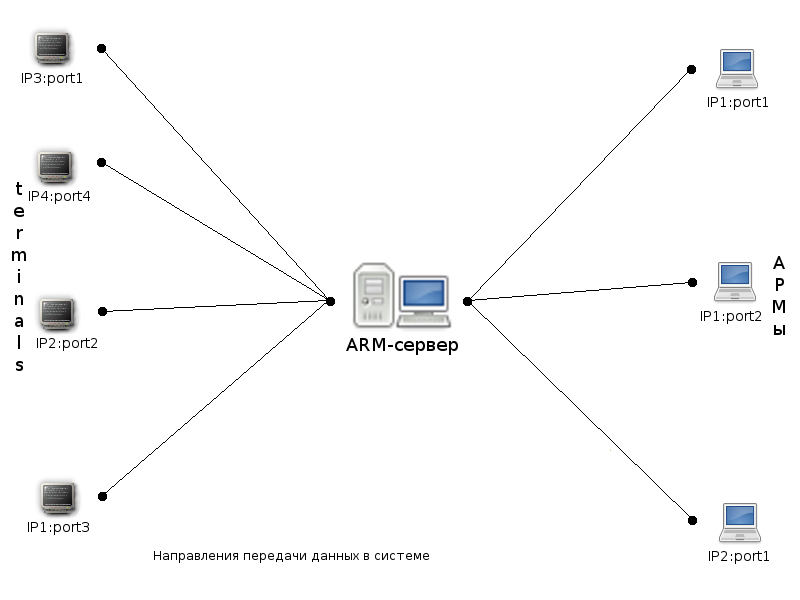
\includegraphics[scale=0.5]{./system_scheme.png}

%---------------------------------------------------------------------------

Типы пакетов:
\begin{itemize}
\item сервисные пакеты (могут рассылаться всеми членами сети):
	\begin{itemize}
	\item keep-alive ping\footnote{Вроде бы что-то вроде этого уже реализовано в протоколе TCP. Если оно меня удовлетворит -- 
	выкину keep-alive ping отсюда.}
	\item пакет с error code 
	\end{itemize}
\item пакеты с данными с датчиков (terminal $\Rightarrow$ АРМ)
\item пакеты с управляющими командами (АРМ $\Rightarrow$ terminal)
\end{itemize}

%---------------------------------------------------------------------------

\section*{Формат пакетов:}
\subsection*{Заголовок, общий для всех типов пакетов:}

\setlength{\bitwidth}{1.2cm}
\scriptsize{
\begin{bytefield}{7}
\bitheader{0,1-4,5-6}\\
\bitbox{1}{{байт типа \\ пакета}} & \bitbox{4}{IP адрес} & \bitbox{2}{port}\\
\bitbox[r]{1}{{}} & \bitbox{6}{адрес получателя пакета}\\
\end{bytefield}
}

\normalsize{}
\setlength{\bitwidth}{1.0cm}
Пример формирования адреса получателя для 192.168.50.1:26000 \\
\\
\begin{bytefield}{7}
\bitheader{0,1,2,3,4,5-6}\\
\bitbox{1}{0x--} & \bitbox{1}{0xc0} & \bitbox{1}{0xa8} & \bitbox{1}{0x32} & \bitbox{1}{0x01} & \bitbox{2}{0x6590}\\
\end{bytefield}

Возможные байты типа пакета:
\begin{description}
\item[0xff] сервисный пакет
\item[0xda] пакет с данными
\item[0xc0] пакет с управляющими командами
\end{description}

Для broadcast-пакетов поля IP:port имеют следующий вид:
\begin{itemize}
\item широковещательная рассылка для терминалов:\\
\\
\begin{bytefield}{7}
\bitheader{0,1-4,5-6}\\
\bitbox{1}{0x--} & \bitbox{1}{0x00} & \bitbox{1}{0x00} & \bitbox{1}{0x00} & \bitbox{1}{0x00} & \bitbox{2}{0xffff}\\
\end{bytefield}

\item широковещательная рассылка для АРМ:\\
\\
\begin{bytefield}{7}
\bitheader{0,1-4,5-6}\\
\bitbox{1}{0x--} & \bitbox{1}{0x00} & \bitbox{1}{0x00} & \bitbox{1}{0x00} & \bitbox{1}{0x00} & \bitbox{2}{0x0000}\\
\end{bytefield}
\end{itemize}

%---------------------------------------------------------------------------

\section*{Данные, специфичные для каждого типа пакетов:}
\subsection*{Сервисные пакеты}

\begin{bytefield}{8}
\bitheader{0-3,4-5,6-7}\\
\bitbox{4}{IP отправителя} & \bitbox{2}{порт отправителя} & \bitbox{1}{error code} \bitbox{1}{0x00}\\
\end{bytefield}

Для keep-alive ping error code должен быть равным \texttt{0x00}. Этот пакет должен посылаться сервером клиенту, каждые 10 минут. 
Далее клиент должен немедленно ответить таким же пакетом серверу. Максимальное время ожидания ответа от 
клиента -- 10 минут. Если ответа нет -- клиент должен быть немедленно отключен от сервера.

Остальные возможные значения error code:
\begin{description}
\item[0xcc] не совпадает CRC блока данных с CRC, присланной в пакете
\item[0x71] не совпадает адрес получателя, присланный в пакете, с реальным адресом получателя 
(используется терминалами и АРМ).
\item[0x82] адрес отправителя некорректен (не существует).
\item[0x72] адрес получателя некорректен (не существует).
\item[0x1c] некорректный код команды.
\item[0xd0] нулевой размер блока с данными.
\item[0xff] неизвестная ошибка.
\item[0xbc] некорректно указана цель широковещательной рассылки пакетов.
\item[0x27] некорректно указан тип пакета.
\item[0x01] null-terminate байт не встречен там, где ожидается.
\end{description}

\subsection*{Пакеты с командами от АРМ}
\begin{bytefield}{8}
\bitheader{0-3,4-5,6-7}\\
\bitbox{4}{IP отправителя} & \bitbox{2}{порт отправителя} & \bitbox{1}{command code} \bitbox{1}{0x00}\\
\end{bytefield}

Возможные значения command code:
\begin{description}
\item[0xdc] запросить пакет с данными от терминала.
%\item[0xc2] переоткрыть сетевое соединение терминала с сервером (успешное выполнение и работоспособность терминала 
%после этого не гарантируются).
\item[0xf2] остановить работу терминала (дальнейшая работа с терминалом невозможна, до его включения).
\end{description}

\subsection*{Пакеты с данными от терминалов}
\small{
\begin{bytefield}{15}
\bitheader{0-3,4-5,6-9,10-11,12-13,14}\\
\bitbox{4}{IP отправителя} & \bitbox{2}{порт отправителя} & \bitbox{4}{размер блока данных} & \bitbox{2}{блок данных} & \bitbox{2}{CRC} & \bitbox{1}{0x00}\\
\end{bytefield}
}
\normalsize{}

Максимальный размер блока данных (указывается размер уже закриптованного блока, который и посылается в составе пакета): 256 Мб. Содержимое блока 
данных не является жестко заданным -- оно определяется и интерпретируется программным обеспечением терминала и АРМ, что позволяет адаптировать 
протокол под определенные цели. Контрольная сумма вычисляется по табличному алгоритму CRC16 (наиболее быстрый, см. 
\texttt{http://ru.wikipedia.org/wiki/CRC}). CRC вычисляется у незашифрованного блока данных.


%---------------------------------------------------------------------------

\section*{Приоритеты пакетов}
Каждый передаваемый пакет имеет свой приоритет. Пакеты с большим приоритетом, доставляются быстрее из пакетов с 
одинаковыми адресами доставки. Приоритеты расставляются в зависимости от типа пакета; типы приведены по убыванию 
их приоритета:
\begin{itemize}
\item сервисные сообщения
\item данные от терминалов
\item команды от АРМ
\end{itemize}
Два последних пункта могут меняться в зависимости от задачи. Для команд от АРМ приоритеты выставляются в зависимости 
от кода операции. Максимальный приоритет у кода \texttt{0xdc}, затем \texttt{0xf2} -- это обеспечивает 
гарантированное исполнение служебных команд до остановки терминала.

%---------------------------------------------------------------------------

\section*{Взаимодействие и алгоритмы работы узлов в сети}
\subsection*{Клиент -- терминал}
При получении управляющего пакета, клиент выполняет содержащееся в нем действие, например отсылает пакет с данными. 
При получении сервисного пакета, клиент выполняет меры по коррекции ошибки; как минимум заносит код ошибки в лог. Если 
получен сервисный пакет с keep-alive ping, то немедленно отвечаем отправителю таким же пакетом. Если внезапно пришел пакет с 
данными -- игнорируем его.

Возможный алгоритм работы узла:
\begin{enumerate}
\item Подключаемся к серверу.
\item Ждем команду от АРМ. Если команда не пришла в течение \texttt{TIME} секунд -- прерываемся. Повторяем попытку 
прочитать команду \texttt{NRETRY} раз. Если это так и не получилось, то переходим к следующему пункту.
\item Проверяем буфер отправки данных -- если он не пуст -- отправляем данные из него по сети.
\item Переходим к пункту \#2.
\item Отключаемся от сервера.
\end{enumerate}

\subsection*{Клиент -- АРМ}
При получении пакета с данными, клиент выводит полученную информацию на экран пользователю или заносит в лог. 
При получении сервисного пакетa, клиент выполянет меры по коррекции ошибки или, как минимум, выводит информацию об 
ошибке на экран и заносит ее в лог. При получении управляющего пакета, клиент игнорирует его.

Действия, при получении сервисного пакета с keep-alive ping аналогичны тем же у терминала.

Возможный алгоритм работы узла:
\begin{enumerate}
\item Подключаемся к серверу.
\item Проверяем буфер отправки команд. Если он не пуст -- отсылаем команды из него терминалам.
\item Ждем данные от терминалов. Если данные не пришли в течение \texttt{TIME} секунд -- прерываемся. 
Повторяем попытку прочесть данные \texttt{NRETRY} раз. Если не получилось -- переходим к следующему шагу.

Значения \texttt{TIME} и \texttt{NRETRY} должны быть достаточно маленькими, чтобы не создавать задержек при 
отсылке команд.
\item Переходим к пункту \#2
\item Отключаемся от сервера.
\end{enumerate}

\subsection*{Сервер}
Сервер должен обеспечивать простую пересылку пакетов между клиентами в сети, руководствуясь указанным в заголовке 
пакета адресом получателя. Если нужно послать broadcast-пакет, он рассылается всем клиентам указанной группы.

Возможный алгоритм работы сервера:
\begin{enumerate}
\item Запускаются 2 прослушивающих сокета -- отдельно один для клиента-АРМ и один для клиента-терминала.
\item Подключившиеся клиенты ставятся в соответствующие им очереди на ожидание событий "\texttt{ready to read}" и 
"\texttt{ready to write}".
\item Сокеты из набора для АРМ проверяются на возникновение события "\texttt{ready to read}". Если оно произошло -- 
читаем полученный пакет в буфер для АРМ.
\item Сокеты из набора для терминалов проверяются на возникновение события "\texttt{ready to read}". Если оно произошло -- 
читаем полученный пакет в буфер для терминалов.
\item Запускаем функции, упорядочивающие пакеты в определенном буфере соответственно их приоритетам.
\item Сокеты из набора для терминалов проверяются на возникновение события "\texttt{ready to write}". Если оно произошло -- 
в соответствующем буфере пакетов ищутся пакеты с соответствующим адресом получателя и отправляются по сети.
\item Сокеты из набора для АРМ проверяются на возникновение события "\texttt{ready to write}". Если оно произошло -- 
в соответствующем буфере пакетов ищутся пакеты с соответствующим адресом получателя и отправляются по сети.
\item Переходим к шагу \#2.
\item Закрываем все сокеты, завершаем сервер.
\end{enumerate}

%---------------------------------------------------------------------------

\section*{Работа протокола с точки зрения семиуровневой сетевой модели OSI}
Отправкой и получением пакетов занимается сеансовый уровень. Ошибка, произошедшая при получении пакета, на любом из 
представленных трех уровней, вызывает прекращение обработки пакета и формирование кода ошибки и посылку сервисного 
пакета с этим кодом по сети.

Сервер, работает на сеансовом уровне.

\subsection*{Прикладной уровень}
Формируем блок данных или код ошибки/команды. Все двух- четырехбайтовые значения должны посылаться в 
сетевом порядке байтов.

\subsection*{Представительский уровень}
У блока данных, полученного с прикладного уровня, вычисляется CRC, он шифруется и вычисляется его размер. Вся эта информация 
добавляется в пакет. Код ошибки/команды, полученный с предыдущего уровня, не модифицируется.

Далее, к пакету добавляется адрес отправителя и null-terminate байт.

\subsection*{Сеансовый уровень}
К пакету, сформированному на представительском уровне, добавляется адрес получателя пакета и байт типа пакета. 
Затем, уже сформированный пакет отправляется в сеть.
\end{document}

